% This file is generated by the MATLAB m-file laprint.m. It can be included
% into LaTeX documents using the packages graphicx, color and psfrag.
% It is accompanied by a postscript file. A sample LaTeX file is:
%    \documentclass{article}\usepackage{graphicx,color,psfrag}
%    \begin{document}% This file is generated by the MATLAB m-file laprint.m. It can be included
% into LaTeX documents using the packages graphicx, color and psfrag.
% It is accompanied by a postscript file. A sample LaTeX file is:
%    \documentclass{article}\usepackage{graphicx,color,psfrag}
%    \begin{document}% This file is generated by the MATLAB m-file laprint.m. It can be included
% into LaTeX documents using the packages graphicx, color and psfrag.
% It is accompanied by a postscript file. A sample LaTeX file is:
%    \documentclass{article}\usepackage{graphicx,color,psfrag}
%    \begin{document}% This file is generated by the MATLAB m-file laprint.m. It can be included
% into LaTeX documents using the packages graphicx, color and psfrag.
% It is accompanied by a postscript file. A sample LaTeX file is:
%    \documentclass{article}\usepackage{graphicx,color,psfrag}
%    \begin{document}\input{fig_thr_est_time_tradeoff_fading_pres}\end{document}
% See http://www.mathworks.de/matlabcentral/fileexchange/loadFile.do?objectId=4638
% for recent versions of laprint.m.
%
% created by:           LaPrint version 3.16 (13.9.2004)
% created on:           22-May-2015 11:07:55
% eps bounding box:     12 cm x 9 cm
% comment:              
%
%\begin{psfrags}%
%\psfragscanon%
%
% text strings:
\psfrag{s08}[b][b]{\fontsize{5.5}{8.25}\fontseries{m}\mathversion{normal}\fontshape{n}\selectfont \color[rgb]{0,0,1}\setlength{\tabcolsep}{0pt}\begin{tabular}{c}$\ers$ = [bits/sec/Hz]\end{tabular}}%
\psfrag{s09}[t][t]{\fontsize{5.5}{8.25}\fontseries{m}\mathversion{normal}\fontshape{n}\selectfont \color[rgb]{0,0,0}\setlength{\tabcolsep}{0pt}\begin{tabular}{c}$\tau$ = [ms]\end{tabular}}%
\psfrag{s13}[][]{\fontsize{10}{15}\fontseries{m}\mathversion{normal}\fontshape{n}\selectfont \color[rgb]{0,0,0}\setlength{\tabcolsep}{0pt}\begin{tabular}{c} \end{tabular}}%
\psfrag{s14}[][]{\fontsize{10}{15}\fontseries{m}\mathversion{normal}\fontshape{n}\selectfont \color[rgb]{0,0,0}\setlength{\tabcolsep}{0pt}\begin{tabular}{c} \end{tabular}}%
\psfrag{s16}[t][t]{\fontsize{5.5}{8.25}\fontseries{m}\mathversion{normal}\fontshape{n}\selectfont \color[rgb]{0,0.5,0}\setlength{\tabcolsep}{0pt}\begin{tabular}{c}$\pc$\end{tabular}}%
\psfrag{s17}[t][t]{\fontsize{5.5}{8.25}\fontseries{m}\mathversion{normal}\fontshape{n}\selectfont \color[rgb]{0,0,0}\setlength{\tabcolsep}{0pt}\begin{tabular}{c}$\tau$ = [ms]\end{tabular}}%
\psfrag{s18}[l][l]{\fontsize{5.5}{8.25}\fontseries{m}\mathversion{normal}\fontshape{n}\selectfont \color[rgb]{0,0,0}theory}%
\psfrag{s19}[l][l]{\fontsize{5.5}{8.25}\fontseries{m}\mathversion{normal}\fontshape{n}\selectfont \color[rgb]{0,0,0}$\ers$}%
\psfrag{s20}[l][l]{\fontsize{5.5}{8.25}\fontseries{m}\mathversion{normal}\fontshape{n}\selectfont \color[rgb]{0,0,0}$\pc$}%
\psfrag{s21}[l][l]{\fontsize{5.5}{8.25}\fontseries{m}\mathversion{normal}\fontshape{n}\selectfont \color[rgb]{0,0,0}(6)}%
\psfrag{s22}[l][l]{\fontsize{5.5}{8.25}\fontseries{m}\mathversion{normal}\fontshape{n}\selectfont \color[rgb]{0,0,0}theory}%
%
% axes font properties:
\fontsize{5.5}{8.25}\fontseries{m}\mathversion{normal}%
\fontshape{n}\selectfont%
%
% xticklabels:
\psfrag{x01}[t][t]{$10^{-2}$}%
\psfrag{x02}[t][t]{$10^{-1}$}%
\psfrag{x03}[t][t]{$10^{0}$}%
\psfrag{x04}[t][t]{$10^{1}$}%
\psfrag{x05}[t][t]{$10^{-2}$}%
\psfrag{x06}[t][t]{$10^{-1}$}%
\psfrag{x07}[t][t]{$10^{0}$}%
\psfrag{x08}[t][t]{$10^{1}$}%
%
% yticklabels:
\psfrag{v01}[l][l]{0.016}%
\psfrag{v02}[l][l]{0.019}%
\psfrag{v03}[l][l]{0.022}%
\psfrag{v04}[l][l]{0.026}%
\psfrag{v05}[l][l]{0.029}%
\psfrag{v06}[l][l]{0.032}%
\psfrag{v07}[r][r]{2.58}%
\psfrag{v08}[r][r]{2.86}%
\psfrag{v09}[r][r]{3.15}%
\psfrag{v10}[r][r]{3.43}%
\psfrag{v11}[r][r]{3.71}%
%
% Figure:
%\resizebox{6cm}{!}{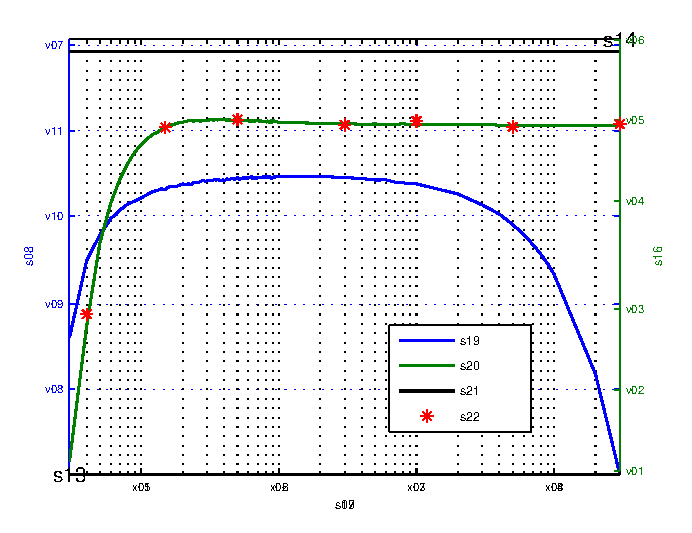
\includegraphics{fig_thr_est_time_tradeoff_fading_pres.eps}}%
%\end{psfrags}%
%
% End fig_thr_est_time_tradeoff_fading_pres.tex
\end{document}
% See http://www.mathworks.de/matlabcentral/fileexchange/loadFile.do?objectId=4638
% for recent versions of laprint.m.
%
% created by:           LaPrint version 3.16 (13.9.2004)
% created on:           22-May-2015 11:07:55
% eps bounding box:     12 cm x 9 cm
% comment:              
%
%\begin{psfrags}%
%\psfragscanon%
%
% text strings:
\psfrag{s08}[b][b]{\fontsize{5.5}{8.25}\fontseries{m}\mathversion{normal}\fontshape{n}\selectfont \color[rgb]{0,0,1}\setlength{\tabcolsep}{0pt}\begin{tabular}{c}$\ers$ = [bits/sec/Hz]\end{tabular}}%
\psfrag{s09}[t][t]{\fontsize{5.5}{8.25}\fontseries{m}\mathversion{normal}\fontshape{n}\selectfont \color[rgb]{0,0,0}\setlength{\tabcolsep}{0pt}\begin{tabular}{c}$\tau$ = [ms]\end{tabular}}%
\psfrag{s13}[][]{\fontsize{10}{15}\fontseries{m}\mathversion{normal}\fontshape{n}\selectfont \color[rgb]{0,0,0}\setlength{\tabcolsep}{0pt}\begin{tabular}{c} \end{tabular}}%
\psfrag{s14}[][]{\fontsize{10}{15}\fontseries{m}\mathversion{normal}\fontshape{n}\selectfont \color[rgb]{0,0,0}\setlength{\tabcolsep}{0pt}\begin{tabular}{c} \end{tabular}}%
\psfrag{s16}[t][t]{\fontsize{5.5}{8.25}\fontseries{m}\mathversion{normal}\fontshape{n}\selectfont \color[rgb]{0,0.5,0}\setlength{\tabcolsep}{0pt}\begin{tabular}{c}$\pc$\end{tabular}}%
\psfrag{s17}[t][t]{\fontsize{5.5}{8.25}\fontseries{m}\mathversion{normal}\fontshape{n}\selectfont \color[rgb]{0,0,0}\setlength{\tabcolsep}{0pt}\begin{tabular}{c}$\tau$ = [ms]\end{tabular}}%
\psfrag{s18}[l][l]{\fontsize{5.5}{8.25}\fontseries{m}\mathversion{normal}\fontshape{n}\selectfont \color[rgb]{0,0,0}theory}%
\psfrag{s19}[l][l]{\fontsize{5.5}{8.25}\fontseries{m}\mathversion{normal}\fontshape{n}\selectfont \color[rgb]{0,0,0}$\ers$}%
\psfrag{s20}[l][l]{\fontsize{5.5}{8.25}\fontseries{m}\mathversion{normal}\fontshape{n}\selectfont \color[rgb]{0,0,0}$\pc$}%
\psfrag{s21}[l][l]{\fontsize{5.5}{8.25}\fontseries{m}\mathversion{normal}\fontshape{n}\selectfont \color[rgb]{0,0,0}(6)}%
\psfrag{s22}[l][l]{\fontsize{5.5}{8.25}\fontseries{m}\mathversion{normal}\fontshape{n}\selectfont \color[rgb]{0,0,0}theory}%
%
% axes font properties:
\fontsize{5.5}{8.25}\fontseries{m}\mathversion{normal}%
\fontshape{n}\selectfont%
%
% xticklabels:
\psfrag{x01}[t][t]{$10^{-2}$}%
\psfrag{x02}[t][t]{$10^{-1}$}%
\psfrag{x03}[t][t]{$10^{0}$}%
\psfrag{x04}[t][t]{$10^{1}$}%
\psfrag{x05}[t][t]{$10^{-2}$}%
\psfrag{x06}[t][t]{$10^{-1}$}%
\psfrag{x07}[t][t]{$10^{0}$}%
\psfrag{x08}[t][t]{$10^{1}$}%
%
% yticklabels:
\psfrag{v01}[l][l]{0.016}%
\psfrag{v02}[l][l]{0.019}%
\psfrag{v03}[l][l]{0.022}%
\psfrag{v04}[l][l]{0.026}%
\psfrag{v05}[l][l]{0.029}%
\psfrag{v06}[l][l]{0.032}%
\psfrag{v07}[r][r]{2.58}%
\psfrag{v08}[r][r]{2.86}%
\psfrag{v09}[r][r]{3.15}%
\psfrag{v10}[r][r]{3.43}%
\psfrag{v11}[r][r]{3.71}%
%
% Figure:
%\resizebox{6cm}{!}{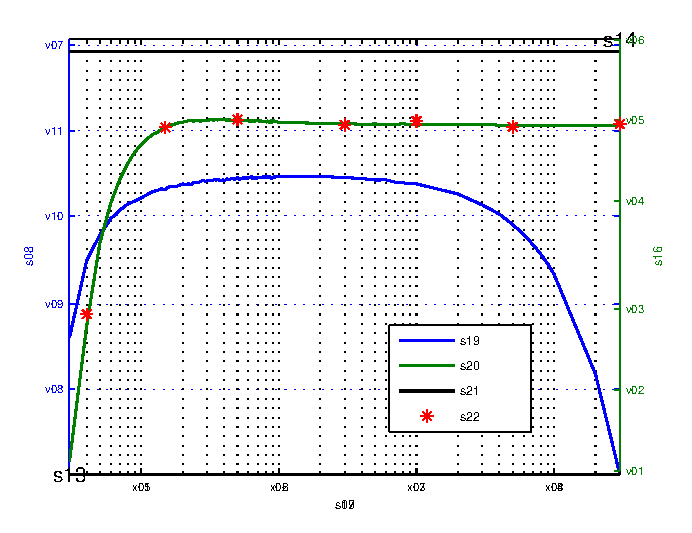
\includegraphics{fig_thr_est_time_tradeoff_fading_pres.eps}}%
%\end{psfrags}%
%
% End fig_thr_est_time_tradeoff_fading_pres.tex
\end{document}
% See http://www.mathworks.de/matlabcentral/fileexchange/loadFile.do?objectId=4638
% for recent versions of laprint.m.
%
% created by:           LaPrint version 3.16 (13.9.2004)
% created on:           22-May-2015 11:07:55
% eps bounding box:     12 cm x 9 cm
% comment:              
%
%\begin{psfrags}%
%\psfragscanon%
%
% text strings:
\psfrag{s08}[b][b]{\fontsize{5.5}{8.25}\fontseries{m}\mathversion{normal}\fontshape{n}\selectfont \color[rgb]{0,0,1}\setlength{\tabcolsep}{0pt}\begin{tabular}{c}$\ers$ = [bits/sec/Hz]\end{tabular}}%
\psfrag{s09}[t][t]{\fontsize{5.5}{8.25}\fontseries{m}\mathversion{normal}\fontshape{n}\selectfont \color[rgb]{0,0,0}\setlength{\tabcolsep}{0pt}\begin{tabular}{c}$\tau$ = [ms]\end{tabular}}%
\psfrag{s13}[][]{\fontsize{10}{15}\fontseries{m}\mathversion{normal}\fontshape{n}\selectfont \color[rgb]{0,0,0}\setlength{\tabcolsep}{0pt}\begin{tabular}{c} \end{tabular}}%
\psfrag{s14}[][]{\fontsize{10}{15}\fontseries{m}\mathversion{normal}\fontshape{n}\selectfont \color[rgb]{0,0,0}\setlength{\tabcolsep}{0pt}\begin{tabular}{c} \end{tabular}}%
\psfrag{s16}[t][t]{\fontsize{5.5}{8.25}\fontseries{m}\mathversion{normal}\fontshape{n}\selectfont \color[rgb]{0,0.5,0}\setlength{\tabcolsep}{0pt}\begin{tabular}{c}$\pc$\end{tabular}}%
\psfrag{s17}[t][t]{\fontsize{5.5}{8.25}\fontseries{m}\mathversion{normal}\fontshape{n}\selectfont \color[rgb]{0,0,0}\setlength{\tabcolsep}{0pt}\begin{tabular}{c}$\tau$ = [ms]\end{tabular}}%
\psfrag{s18}[l][l]{\fontsize{5.5}{8.25}\fontseries{m}\mathversion{normal}\fontshape{n}\selectfont \color[rgb]{0,0,0}theory}%
\psfrag{s19}[l][l]{\fontsize{5.5}{8.25}\fontseries{m}\mathversion{normal}\fontshape{n}\selectfont \color[rgb]{0,0,0}$\ers$}%
\psfrag{s20}[l][l]{\fontsize{5.5}{8.25}\fontseries{m}\mathversion{normal}\fontshape{n}\selectfont \color[rgb]{0,0,0}$\pc$}%
\psfrag{s21}[l][l]{\fontsize{5.5}{8.25}\fontseries{m}\mathversion{normal}\fontshape{n}\selectfont \color[rgb]{0,0,0}(6)}%
\psfrag{s22}[l][l]{\fontsize{5.5}{8.25}\fontseries{m}\mathversion{normal}\fontshape{n}\selectfont \color[rgb]{0,0,0}theory}%
%
% axes font properties:
\fontsize{5.5}{8.25}\fontseries{m}\mathversion{normal}%
\fontshape{n}\selectfont%
%
% xticklabels:
\psfrag{x01}[t][t]{$10^{-2}$}%
\psfrag{x02}[t][t]{$10^{-1}$}%
\psfrag{x03}[t][t]{$10^{0}$}%
\psfrag{x04}[t][t]{$10^{1}$}%
\psfrag{x05}[t][t]{$10^{-2}$}%
\psfrag{x06}[t][t]{$10^{-1}$}%
\psfrag{x07}[t][t]{$10^{0}$}%
\psfrag{x08}[t][t]{$10^{1}$}%
%
% yticklabels:
\psfrag{v01}[l][l]{0.016}%
\psfrag{v02}[l][l]{0.019}%
\psfrag{v03}[l][l]{0.022}%
\psfrag{v04}[l][l]{0.026}%
\psfrag{v05}[l][l]{0.029}%
\psfrag{v06}[l][l]{0.032}%
\psfrag{v07}[r][r]{2.58}%
\psfrag{v08}[r][r]{2.86}%
\psfrag{v09}[r][r]{3.15}%
\psfrag{v10}[r][r]{3.43}%
\psfrag{v11}[r][r]{3.71}%
%
% Figure:
%\resizebox{6cm}{!}{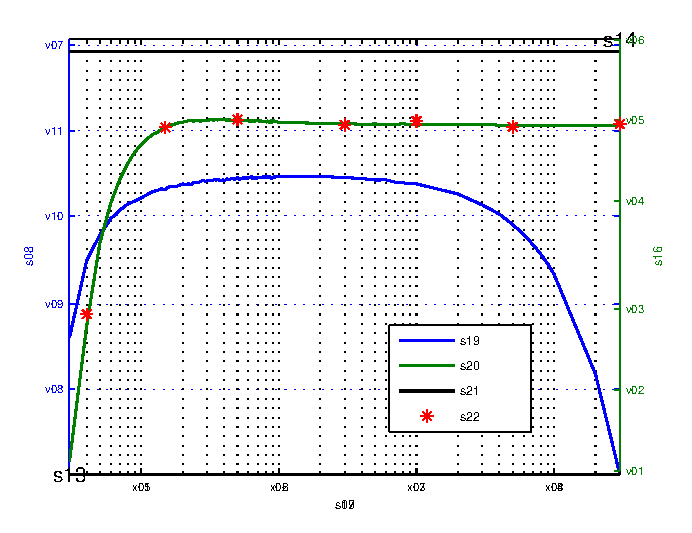
\includegraphics{fig_thr_est_time_tradeoff_fading_pres.eps}}%
%\end{psfrags}%
%
% End fig_thr_est_time_tradeoff_fading_pres.tex
\end{document}
% See http://www.mathworks.de/matlabcentral/fileexchange/loadFile.do?objectId=4638
% for recent versions of laprint.m.
%
% created by:           LaPrint version 3.16 (13.9.2004)
% created on:           22-May-2015 11:07:55
% eps bounding box:     12 cm x 9 cm
% comment:              
%
%\begin{psfrags}%
%\psfragscanon%
%
% text strings:
\psfrag{s08}[b][b]{\fontsize{5.5}{8.25}\fontseries{m}\mathversion{normal}\fontshape{n}\selectfont \color[rgb]{0,0,1}\setlength{\tabcolsep}{0pt}\begin{tabular}{c}$\ers$ = [bits/sec/Hz]\end{tabular}}%
\psfrag{s09}[t][t]{\fontsize{5.5}{8.25}\fontseries{m}\mathversion{normal}\fontshape{n}\selectfont \color[rgb]{0,0,0}\setlength{\tabcolsep}{0pt}\begin{tabular}{c}$\tau$ = [ms]\end{tabular}}%
\psfrag{s13}[][]{\fontsize{10}{15}\fontseries{m}\mathversion{normal}\fontshape{n}\selectfont \color[rgb]{0,0,0}\setlength{\tabcolsep}{0pt}\begin{tabular}{c} \end{tabular}}%
\psfrag{s14}[][]{\fontsize{10}{15}\fontseries{m}\mathversion{normal}\fontshape{n}\selectfont \color[rgb]{0,0,0}\setlength{\tabcolsep}{0pt}\begin{tabular}{c} \end{tabular}}%
\psfrag{s16}[t][t]{\fontsize{5.5}{8.25}\fontseries{m}\mathversion{normal}\fontshape{n}\selectfont \color[rgb]{0,0.5,0}\setlength{\tabcolsep}{0pt}\begin{tabular}{c}$\pc$\end{tabular}}%
\psfrag{s17}[t][t]{\fontsize{5.5}{8.25}\fontseries{m}\mathversion{normal}\fontshape{n}\selectfont \color[rgb]{0,0,0}\setlength{\tabcolsep}{0pt}\begin{tabular}{c}$\tau$ = [ms]\end{tabular}}%
\psfrag{s18}[l][l]{\fontsize{5.5}{8.25}\fontseries{m}\mathversion{normal}\fontshape{n}\selectfont \color[rgb]{0,0,0}theory}%
\psfrag{s19}[l][l]{\fontsize{5.5}{8.25}\fontseries{m}\mathversion{normal}\fontshape{n}\selectfont \color[rgb]{0,0,0}$\ers$}%
\psfrag{s20}[l][l]{\fontsize{5.5}{8.25}\fontseries{m}\mathversion{normal}\fontshape{n}\selectfont \color[rgb]{0,0,0}$\pc$}%
\psfrag{s21}[l][l]{\fontsize{5.5}{8.25}\fontseries{m}\mathversion{normal}\fontshape{n}\selectfont \color[rgb]{0,0,0}(6)}%
\psfrag{s22}[l][l]{\fontsize{5.5}{8.25}\fontseries{m}\mathversion{normal}\fontshape{n}\selectfont \color[rgb]{0,0,0}theory}%
%
% axes font properties:
\fontsize{5.5}{8.25}\fontseries{m}\mathversion{normal}%
\fontshape{n}\selectfont%
%
% xticklabels:
\psfrag{x01}[t][t]{$10^{-2}$}%
\psfrag{x02}[t][t]{$10^{-1}$}%
\psfrag{x03}[t][t]{$10^{0}$}%
\psfrag{x04}[t][t]{$10^{1}$}%
\psfrag{x05}[t][t]{$10^{-2}$}%
\psfrag{x06}[t][t]{$10^{-1}$}%
\psfrag{x07}[t][t]{$10^{0}$}%
\psfrag{x08}[t][t]{$10^{1}$}%
%
% yticklabels:
\psfrag{v01}[l][l]{0.016}%
\psfrag{v02}[l][l]{0.019}%
\psfrag{v03}[l][l]{0.022}%
\psfrag{v04}[l][l]{0.026}%
\psfrag{v05}[l][l]{0.029}%
\psfrag{v06}[l][l]{0.032}%
\psfrag{v07}[r][r]{2.58}%
\psfrag{v08}[r][r]{2.86}%
\psfrag{v09}[r][r]{3.15}%
\psfrag{v10}[r][r]{3.43}%
\psfrag{v11}[r][r]{3.71}%
%
% Figure:
%\resizebox{6cm}{!}{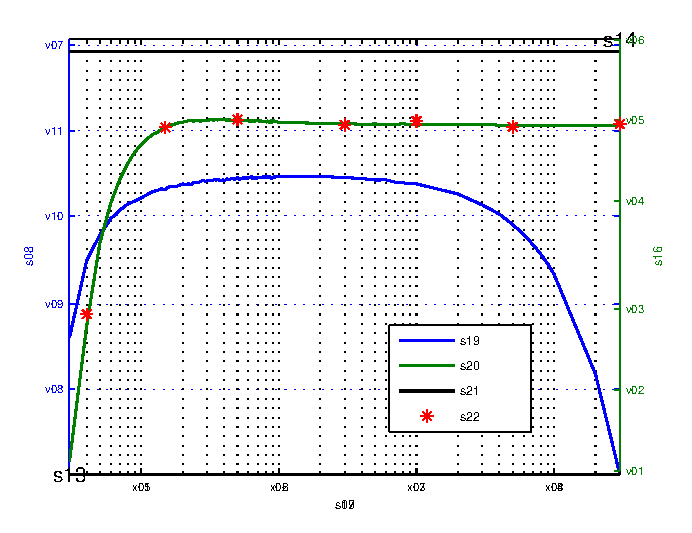
\includegraphics{fig_thr_est_time_tradeoff_fading_pres.eps}}%
%\end{psfrags}%
%
% End fig_thr_est_time_tradeoff_fading_pres.tex
